\chapter{Métodos inferiores}\label{cap:inferiores}
Neste capítulo, são apresentados quatro algoritmos básicos para o problema da ordenação. Esses algoritmos são chamados de inferiores por serem simples, intuitivos e, principalmente, por apresentarem, no mínimo, complexidade temporal quadrática nos casos médio e pior.

\section{Bolha}
O algoritmo Bolha é um dos algoritmos mais simples para o problema da ordenação. Ele consistem em percorrer várias vezes o vetor, comparando elementos adjacentes e trocando-os de posição caso estejam fora da ordem desejada. Nesse processo, os elementos flutuam para suas posições finais. Em outras palavras, ``[...]  os elementos da lista são movidos para as posições adequadas de forma contínua, assim como uma bolha move-se num líquido. Se um elemento está inicialmente numa posição i e, para que a lista fique ordenada, ele deve ocupar a posição j, então ele terá que passar por todas as posições entre i e j.'' \cite[p.8]{viana2011pesquisa}.

\lstinputlisting[language=C]{codigos/inf/1_bolha.txt}

Esta versão do algoritmo Bolha é também conhecida como ``Bolha com Flag'', por conta do uso da variável \textit{trocou}. Perceba que, sem essa variável, o algoritmo continua funcionando da mesma forma; porém o laço externo executará sempre $n - 1$ iterações, mesmo que o vetor fique ordenado antes.

Observe que o algoritmo Bolha oferece uma ordenação estável, pois, quando dois elementos adjacentes são iguais, eles não são trocados.

\subsection*{Corretude}
Ao final de uma iteração do laço externo, o maior elemento de $v[0..i]$ estará na posição $i$. Dessa forma, ao final da primeira iteração, o maior elemento do vetor estará na posição $n - 1$; ao final da segunda iteração, o segundo maior estará na posição $n - 2$, e assim por diante. Portanto, o algoritmo Bolha é correto.

\subsection*{Desempenho}
Em termos de consumo de memória adicional, o algoritmo declara apenas três variáveis escalares, sendo duas delas para controle de laço de repetição. Logo, sua complexidade espacial é $\Theta(1)$. Esta observação será omitida para os algoritmos apresentados a seguir que tenham a mesma complexidade espacial.

Já para a complexidade temporal, o melhor caso ocorre quando a entrada já está ordenada em ordem crescente, pois não é realizada nenhuma troca. Exige-se, assim, apenas uma iteração do laço externo, resultando em complexidade $\Theta(n)$.

Por outro lado, o pior caso ocorre quando o menor elemento está na última posição, sendo necessárias exatamente $n - 1$ iterações do laço externo para que ele chegue à primeira posição. Com isso, a quantidade de iterações do laço interno é dada pela seguinte soma:
\begin{equation}\label{eq:1}
    \sum_{i=1}^{n-1} i = \frac{n(n-1)}{2}
\end{equation}
Isso implica em uma complexidade quadrática $\Theta(n^2)$. Em média, a complexidade temporal do algoritmo Bolha é \bigO{n^2}.

\section{Coquetel}
O Coquetel é um algoritmo de ordenação estável que traz a mesma ideia do Bolha, mas com um laço interno adicional. O primeiro laço, assim como no Bolha, itera da esquerda para a direita, empurrando os maiores elementos para o final do vetor, enquanto o segundo itera no outro sentido, empurrando os menores elementos para o início.

\lstinputlisting[language=C]{codigos/inf/2_coquetel.txt}

\subsection*{Corretude}
Ao final de uma iteração do laço externo, o menor e o maior elemento de $v[i..j]$ estarão nas posições $i$ e $j$, respectivamente. Dessa forma, ao final da primeira iteração, o menor elemento estará na posição $0$ e o maior, na posição $n - 1$; na segunda, o segundo menor, na posição $1$, e o segundo maior, na posição $n - 2$, e assim por diante. Esse processo garante que, quando $i \geq j$, o vetor estará ordenado; portanto, o algoritmo é correto.

\subsection*{Desempenho}
Embora as complexidades dos casos melhor, pior e médio continuem sendo, respectivamente, $\Theta(n)$, $\Theta(n^2)$ e \bigO{n^2}, o pior caso do Coquetel é menos frequente, pois ocorre apenas quando a entrada está em ordem decrescente.

\begin{figure}[H]
\Caption{\label{fig:coquetel_it}Coquetel aplicado ao vetor $[n, n-1, ..., 2, 1]$.}
\centering
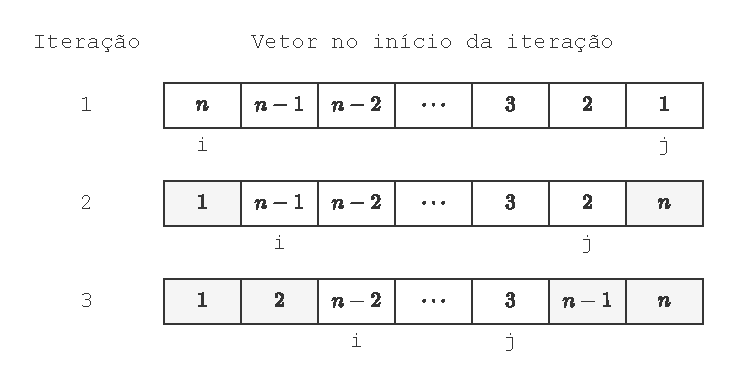
\includegraphics[scale=1.0]{figuras/pdf/coquetel.pdf}
\Fonte{Elaborado pelo autor.}
\end{figure}

Considere então que $T(n)$ é a quantidade total de iterações dos dois laços internos no pior caso. A figura \ref{fig:coquetel_it} ajuda a notar que a seguinte identidade é válida:

\[
T(n) = 
  \begin{cases}
      0,              & n < 2    \\
      T(n-2) + 2n - 3, & n \geq 2 
  \end{cases}
\]

Ao resolver a recorrência mostrada acima, pode-se observar que $T(n)$ é igual a soma \ref{eq:1}. Portanto, os algoritmos Bolha e Coquetel, em seus piores casos, executam exatamente a mesma quantidade de iterações.

\section{Seleção}
O algoritmo Seleção é um método de ordenação instável, como mostra a figura \ref{fig:selecao}. A ideia é bastante simples: execute $n$ iterações; na i-ésima iteração, selecione o i-ésimo menor elemento e coloque-o na posição $i - 1$. Uma propriedade interessante desse algoritmo é que ele realiza o número mínimo possível de trocas para ordenar o vetor.

\lstinputlisting[language=C]{codigos/inf/3_selecao.txt}

\begin{figure}[H]
\Caption{\label{fig:selecao}Seleção aplicado ao vetor \([3, 3, 2, 5]\).}
\centering
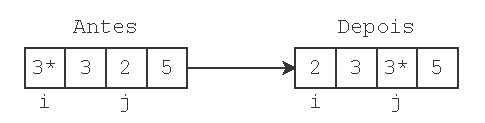
\includegraphics[scale=1.0]{figuras/pdf/selecao.pdf}
\Fonte{Elaborado pelo autor}
\end{figure}

\subsection*{Corretude}
É invariante que, ao final de cada iteração do laço externo, os elementos de $v[0..i]$ já estejam em suas posições definitivas. Portanto, ao final da última iteração, quando $i$ for igual a $n - 1$, o vetor $v[0..n - 1]$ estará ordenado.

\subsection*{Desempenho}
O ponto crítico do algoritmo Seleção é o teste condicional \textit{if} na linha 5. A quantidade de vezes que esse ponto é executado é sempre dada pela soma \ref{eq:1}, ou seja, não há melhor nem pior caso. Portanto, esse algoritmo sempre requer tempo igual a $\Theta(n^2)$.

\section{Inserção}
O algoritmo Inserção é um método de ordenação estável com o melhor desempenho entre os métodos inferiores. A ideia por trás do algoritmo é simples: para $i$ variando de $1$ a $n - 1$, nesta ordem, insira $v[i]$ em $v[0..i - 1]$, de modo que $v[0..i]$ esteja em ordem.

Em especial, o algoritmo Inserção possui complexidade temporal linear para entradas quase ordenadas. Por conta disso, outros algoritmos fazem uso dele como sub-rotina. O Shellsort, por exemplo, utiliza o Inserção para tornar o vetor $h$-ordenado.

\begin{definition}
Para um dado número natural $h > 0$, um vetor $v$ de tamanho $n$ é considerado $h$-ordenado quando $v[i] \leq v[i + h]$, para todo $0 \leq i < n - h$.
\end{definition}

\lstinputlisting[language=C]{codigos/aux/h-ordena.txt}

A implementação do Inserção pode ser idêntica à função H\_Ordena mostrada acima, bastando fazer $h = 1$, pois, nesse caso em particular, um vetor $h$-ordenado é simplesmente um vetor ordenado.

\lstinputlisting[language=C]{codigos/inf/4_insercao.txt}

\subsection*{Corretude}
Ao final de cada iteração do laço externo, o segmento $v[0..i]$ está ordenado. Esse invariante permanece válido durante todas as iterações, inclusive na última. Portanto, ao final do processo, $v[0..n - 1]$ estará ordenado.

\subsection*{Desempenho}
No melhor caso, a complexidade é linear e ocorre quando o vetor já está ordenado, pois a condição do laço interno será sempre falsa. Já o pior caso acontece quando o vetor está em ordem decrescente; nesse cenário, $v[i]$ é sempre inserido na posição $0$. O ponto crítico é a linha 6 e, mais uma vez, a soma \ref{eq:1} determina a quantidade de vezes que essa linha será executada. Portanto, a complexidade no pior caso é $\Theta(n^2)$. Em média, o algoritmo Inserção consome tempo proporcional a \bigO{n^2}.
